\documentclass[a4paper]{jpconf}
\usepackage{graphicx}
\begin{document}
\title{Application of a novel machine learning algorithm in gravitational wave glitch identification}

\author{Ruaridh O'Donnell}

\ead{1002205o@student.gla.c.uk}

\begin{abstract}
    An investigation into wether a recent algorithm would be of use in gravitational wave searches. The algorithm investigated was NuPIC, a recently open sourced algorithm, inspired by layer 2/3 neocortex structure and operation. A detailed description of how this algorithm function is given. A gravitational wave glitch was modelled by a sine gaussian. The algorithm was trained on this glitch and tested to see how well it could differentiate it from background gaussian noise. For low levels of noise nupic was able to differentiate the glitch well, but for higher levels of noise it could not. Additionally some constraints on what kind of training glitch could be used were found and some notes on how the algorithm deals with noise were made. These could be helpful in future work.
    
\end{abstract}
%:This is a tag

\section{Overview}%%%%%%%%%%%%%%%%%%%%%%%%%%%%%%%%%%%%%%%
    The aim of this work was to look at the possible use of a a novel unsupervised machine learning algorithm in the search for gravitational waves. This algorithm is based on an understanding of brain function. There are many challenges in searching for gravitational waves and various machine learning algorithms are starting to be used to tackle them. It is thought that there might be a possible application for this new algorithm.

\section{Background On Gravitational Waves and Detectors}\label{aargh}%%%%%%%%%%%%%
Advances in astronomy typically follow advances in detector technology. Telescopes tuned to wavelengths of light outside the visible spectrum have produced many discoveries beyond what was known only from visible light telescopes. Gravitational waves are predicted to be emitted by many astronomical bodies. If they can be detected then they provide a new method of discovery that is substantially different from electromagnetic radiation. This will allow it to see things that cannot be seen with electromagnetic telescopes.

Detecting gravitational waves produces many technical challenges and thus the detectors are complex. This section will cover a beif overview of the relevant feature of the detectors for this project and also cover some of the ways in which machine learning has been used in this field in the past.

\subsection{Gravitational wave detectors}
quick description of detectors - detectors output time series
The gravitational wave detectors in use today are fundamentally Michelson interferometers. The mirrors at either end of the arms are mounted on test masses that move when gravitational waves pass. The output that measures the passing wave can be thought of as a time series of the power output of the interferometer. In reality modern advanced detectors (such as Advanced LIGO) are considerably more complex but theses details do not need to be understood.

detectors have lots of noise - because waves are tiny
The waves detectable from earth have an extremely small effect on the test masses. The detectors need to have advanced noise removal so much of the work in building the detectors has gone into this. however despite the efforts much noise still remains in the signal. This noise can be broadly split into Gaussian noise and glitches. The glitches can be easily mistaken for actual gravitational wave signals.

\subsection{Past attempts at using machine learning methods in gravitational wave searches}
Machine learning methods are starting to be used in the field of gravitational wave searches. This section contains a summary of some recent efforts. It should be noted that the algorithms used here are substantially different to NuPIC, the algorithm used in this project.

\begin{description}
\item[Inferring Core Collapse Supernova Physics with Gravitational Waves [5]]
There are different possibilities for how supernova evolve. Each would produce a different pattern in the gravitational wave signal. However the waveforms vary enough in each class that that cross-correlation would be impractical. So this paper proposes a method for categorising a signal measured in LIGO into one of the three supernova types using principle component analysis and Bayesian statistics. Principle component analysis has some similarities to the way NuPIC operates so this could be promising.

\item[Noise Artefact Removal Using Machine learning with Gravitational Waves [2]]
These glitches occur frequently enough that they show up in concurrence between two detectors, so it is important to find a way of filtering them out. They often occur in some kind of correlation with other readings taken from the detector. Hence automated machine learning methods can be used to distinguish them from real gravitational wave signals.

They split the data into two categories. The first, glitches that weren't gravitational waves, ie glitches that didn't have any coincidence in other detectors. (they actually just used all the glitches measured and assumed there wasn't any gravitational signals in there). The other was clean data which seems to be random collection of samples from when the gravitational wave channel was quiet.

They achieved similar performance using several different algorithms suggesting that any improvements would be from including additional data in the classification.

\item[Application of Artificial Neural Network to Search for Gravitational-Wave Signals Associated with Short Gamma-Ray Bursts [4]]
This is a fairly basic application of ANNs to categorise glitches.
\end{description}

\section{NuPIC: A Novel Machine Learning Algorithm}%%%%%%%%%%%%%%%%%%%%%%
	NuPIC, or the Numenta Platform for Intelligent Computing is the machine learning algorithm used in this project. It was developed privately by the company Numenta for use in analysis of streaming data. As of SOMETIME 2014 it is in use in a commercial product ``Grok'' but the core algorithm has been open sourced.
		
	This section will go over the main features of this algorithm, followed by a more detailed overview of it's inner workings. This will be illustrated with a simple example. Finally the specific implementation details used in this project will be covered as well as a short analysis of the noise characteristics of the algorithm.

	\subsection{Backround}
		Machine learning algorithms automatically learn patterns in collections of data. This automatic discovery of the underlying statistics in data make them useful across a wide class of domains. Most algorithms operate in a similar manner. They are trained on a collection of data until the patterns are discovered, and then they are used to evaluate new data (that was not in the training set). For example a collection of vectors can be grouped together into classes by a KNN classifier. A new vector can then be evaluated by this algorithm to see which class it belongs to. There is a wide variety in how machine learning algorithms carry out this process. NuPIC was modelled on a theory of how the neocortex (a part of the mammalian brain) functions. This theory is called Hierarchical Temporal Memory (or HTM).
		
		The neocortex is the part of the brain associated with higher intelligent thinking and long term memory. It consists of a sheet across the surface of the brain, approximately 2 mm thick, composed of around six layers. Different areas of the sheet carry out different functions (image processing, language, higher level thought, etc). The neocortex is has very regular structure of cells across these different areas. Vermont Mount-Castle propositioned that despite the different functions, the neocortex is running the same algorithm across all areas. This is the basis of NuPIC. It is the very first part of an implementation of this algorithm.
	
	\subsection{Main features of NuPIC}
		Most machine learning algorithms have a training phase, where they process the data and learn its statistics. Once this phase is over the algorithm does not change. NuPIC operates in a slightly different way that has more in common with biological brains. There is no distinct training phase, instead the data is fed in as a sequence and learning is continuous. For example a time series is fed in sample by sample, with learning happening after every sample.
		
		NuPIC is also unsupervised. Supervised machine learning algorithms try to evaluate data against predefined labels. A common example would training on a collection of images of animals, each labeled with the name of the animal. Then the algorithm would evaluate a new image and come up with the type of animal. NuPIC instead categorises data into categories it chooses. This is how biological brains operate.
		
		As well as learning on each sample, NuPIC forms predictions. This is a major part of the background HTM theory. They happen all the time in the brain and play a role in feedback, stability of representations, robustness to noise and expectedness of input. The import feautres of prediction here are its role in selecting context. When data is fed into NuPIC, it is classified, and a prediction of the next input is formed. This prediction is then used to help classify the next input. Details of this process are in the next section. Prediction allows one to say how unexpected the input is, or how anomalous it is. This anomaly detection was used in the glitch detection.
		
		Internally NuPIC is a neural network. However it the details of this network are more complex than common neural networks.
		
	\subsection{Algorithm details}
		This section borrows heavily from the description in the CLA white paper which contains a much more thorough explanation of the algorithms complete with pseudocode. When data is fed into NuPIC it undergoes three steps. These are:
		\begin{enumerate}
			\item Form a sparse distributed representation of the input
			\item Form a representation of the input in the context of previous inputs
			\item Form a prediction based on the current input in the context of previous inputs
		\end{enumerate}
		\subsubsection{Step 1: Form a sparse distributed representation of the input}
			This step has two subsets. First the input (which in this case could be a sample form a time series (a real number) is converted to a binary vector. This is called encoding. It is not part of the core algorithm but is is necessary to convert the data type of the input into a format that can be used in subsequent steps. It follows that there are different encoders for different data types. For the case of real numbers as used in this project the ``scalar encoder'' was used. A value is converted to a binary vector with a section of bits on in a background of off bits. See FIGREF(in caption: note how similar values map to high overlap) for details. The dimension of the vector and the number of on bits are parameters that do not change between input values.
			
			The next step is so convert this binary vector to a small set of active \emph{columns} contained in a larger set of inactive ones. Consider the following structure FIGREF. The input binary vector from the previous step is inputted at the bottom. Then, in a process covered below, a set of columns become active (usually about 2\% of the total). This set of columns is the sparse distributed representation of the input vector. SDRs have  many useful properties which explain why this step is necessary. For example if you have a set of SDRs then in order to differentiate them you do not need to look at every bit. It is possible to check only a few. This reduces the computations that must be performed. Further, this property allows you to form a superposition of two or more SDRs by or-ing their bits together. The chance of two random SDR overlapping significantly is extremely small. This property proves useful in Step 3 \ref{step3} (semantic meaning and PCA?). 
			
			%Details, ending in results
			Each column has a number of synapses. connecting it to  a large pursuant of the input space. Each of these can be either on or off. When on, they permit the information in the input to pass when off they do not. These act like a mask. For each column you add up all the on input bits that the column can ``see''. Then the top few columns are chosen to become active. This results in about 2\% becoming active. Distributed over the space. Each column corresponds to a ``pattern'' in the input. The set of active columns represents the input in terms of these ``patterns''. Much like a vector can be decomposed into a sum of orthogonal basis vectors. This is what is meant by semantic meaning.
			
		\subsubsection{Step 2: Form a representation of the input in the context of previous inputs}
			This step activates a set of \emph{cells} within each of the columns activated in the last step. Each column is composed of a number of cells which can either be active or inactive. The active columns represent the input, whereas the active cells will represent the input in the context of previous inputs. This is important as an input can mean different things in different contexts. For example in the spoken sequence of words ``I ate a pear'' and ``I have eight pears'' the words ``ate'' and ``eight'' sound exactly the same; they are the same input. Yet, given the context, it is clear they mean different things.
			--bursting--
			In each active column, each cell is activated if it was in a \emph{predicting} state before. See FIGREF for an overview. Predicting cells are explained in the next step.
		\subsubsection{Step 3: Form a prediction based on the current input in the context of previous inputs}\label{step3}
		The predictive cells from last time are activated in this step. As in step one, each cell is connected to collection of other cells by synapses. In this step all the activations on the active synapses are summed to get a total for each cell. Then if this total is above a certain threshold the cell is marked as predicting. Synapses are formed from a cell to cells that become active on the tilmestep before. So if a state occurs that is commonly followed by another state. Cells in state 2 will form connections to cells in state 1. Hence when state 1 is activated, the cells corresponding to state 2 become predicting.
		--Anomaly score--
		
		Sometimes a state is often followed by one of two other states with probabliity half each. In this instance multiple predictions can be formed, predicting both of the next states. This can happen due to the properties of the sparse distributed representations.
		\subsubsection{The Classifier}
			The above three steps represent the core algorithm (excluding encoding). However to form actual predictions of the next numerical input a classifier is used. The predictive cells can be used and fed back through eh synapse connections and the encoder to get back to the actual value. However Numenta found that the classifier produced more accurate predictions.
			
			For each cell a table is kept that records the input values that occurred on the iteration after that cells became active. This is results in a probability distribution for a set of possible next values. For some input, all the active cells are locked at and a prediction is formed for what the next input value will be.
			 
	\subsection{example}
		See notebook for detailed plan.
	
	\subsection{my work}

\section{Glitch Identification}%%%%%%%%%%%%%%%%%%%%%%%%%%%%%%%%%%%%
Intro/reasons for doing this (see big talk plan)
The hypothesis - how I imagined this method working (see big talk plan)
details - the experiment and the precise setup details
Results - The final Graph
Problems
 - overgeneralisation - and consequent investigation
 - low noise tolerance (signal indistinguishable when noise)
 - Trial of training with noise
Discussion - this is very simple but could be applied to other glitches / patterns

\section{Additional Investigations}%%%%%%%%%%%%%%%%%%%%%%%%%%%%%%%%%
\subsection{Gravitational Wave Detector Data}
\subsection{Beta Classification}

\section{Conclusion}%%%%%%%%%%%%%%%%%%%%%%%%%%%%%%%%%%%%%%%
Maybe some things like I had at the end of my talk - general issues in machine learning.

\section*{References} %%%%%%%%%%%%%%%%%%%%%%%%%%%%%%%%%%%%%%
%doesn't the bibtex thing do this for me?
This is some text. This is how you do citations: \cite{}. Type the first few letters and press F5.
This is how you do cross references: \ref{aargh}.

\begin{center}
    \begin{figure}
        \begin{minipage}{40pc}
            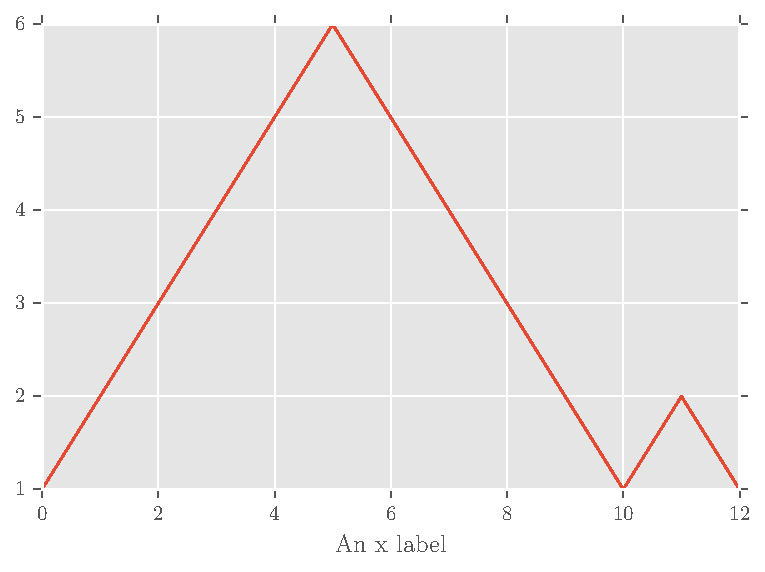
\includegraphics[width=40pc]{testMatplotlibPlot.pdf}
            \caption{A really exciting plot}
        \end{minipage}
    \end{figure}
\end{center}

%%%%%%%%%%%%%%%%%%%%%%%%%%%%%%%%%%%%%%%%%%%%%%%%
%%%%%%%%%%%%%%%%%%%%%%%%%%%%%%%%%%%%%%%%%%%%%%%%
%%%%%%%%%%%%%%%%%%%%%%%%%%%%%%%%%%%%%%%%%%%%%%%%
%%%%%%%%%%%%%%%%%%%%%%%%%%%%%%%%%%%%%%%%%%%%%%%%
%%%%%%%%%%%%%%%%%%%%%%%%%%%%%%%%%%%%%%%%%%%%%%%%
%%%%%%%%%%%%%%%%%%%%%%%%%%%%%%%%%%%%%%%%%%%%%%%%
%%%%%%%%%%%%%%%%%%%%%%%%%%%%%%%%%%%%%%%%%%%%%%%%
%%%%%%%%%%%%%%%%%%%%%%%%%%%%%%%%%%%%%%%%%%%%%%%%
\section{Figures and figure captions}
Figures must be included in the source code of an article at the appropriate place in the text not 
grouped together at the end. 

Each figure should have a brief caption describing it and, if 
necessary, interpreting the various lines and symbols on the figure. 
As much lettering as possible should be removed from the figure itself and 
included in the caption. If a figure has parts, these should be 
labelled ($a$), ($b$), ($c$), etc. 
\Tref{blobs} gives the definitions for describing symbols and lines often
used within figure captions (more symbols are available
when using the optional packages loading the AMS extension fonts).

\begin{table}[h]
\caption{\label{blobs}Control sequences to describe lines and symbols in figure 
captions.}
\begin{center}
\begin{tabular}{lllll}
\br
Control sequence&Output&&Control sequence&Output\\
\mr
\verb"\dotted"&\dotted        &&\verb"\opencircle"&\opencircle\\
\verb"\dashed"&\dashed        &&\verb"\opentriangle"&\opentriangle\\
\verb"\broken"&\broken&&\verb"\opentriangledown"&\opentriangledown\\
\verb"\longbroken"&\longbroken&&\verb"\fullsquare"&\fullsquare\\
\verb"\chain"&\chain          &&\verb"\opensquare"&\opensquare\\
\verb"\dashddot"&\dashddot    &&\verb"\fullcircle"&\fullcircle\\
\verb"\full"&\full            &&\verb"\opendiamond"&\opendiamond\\
\br
\end{tabular}
\end{center}
\end{table}


Authors should try and use the space allocated to them as economically as possible. At times it may be 
convenient to put two figures side by side or the caption at the side of a figure. To put figures side by 
side, within a figure environment, put each figure and its caption into a minipage with an appropriate 
width (e.g. 3in or 18pc if the figures are of equal size) and then separate the figures slightly by adding 
some horizontal space between the two minipages (e.g. \verb"\hspace{.2in}" or \verb"\hspace{1.5pc}". 
To get the caption at the side of the figure add the small horizontal space after the 
\verb"\includegraphics" command and then put the \verb"\caption" within a minipage of the appropriate 
width aligned bottom, i.e. \verb"\begin{minipage}[b]{3in}" etc (see code in this file used to generate 
figures 1--3).

Note that it may be necessary to adjust the size of the figures (using optional arguments to 
\verb"\includegraphics", for instance \verb"[width=3in]") to get you article to fit within your page 
allowance or to obtain good page breaks.

\begin{figure}[h]

\begin{minipage}{14pc}

\includegraphics[width=14pc]{name.eps}
\caption{\label{label}Figure caption for first of two sided figures.}
\end{minipage}

\hspace{2pc}%

\begin{minipage}{14pc}

\includegraphics[width=14pc]{name.eps}
\caption{\label{label}Figure caption for second of two sided figures.}
\end{minipage} 

\end{figure}

\begin{figure}[h]

\includegraphics[width=14pc]{name.eps}\hspace{2pc}%
\begin{minipage}[b]{14pc}\caption{\label{label}Figure caption for a narrow figure where the caption is 
put at the side of the figure.}
\end{minipage}
\end{figure}

Using the graphicx package figures can be included using code such as:
\begin{verbatim}
\begin{figure}
\begin{center}
\includegraphics{file.eps}
\end{center}
\caption{\label{label}Figure caption}
\end{figure}
\end{verbatim}


\section{Preparing your paper}
\verb"jpconf" requires \LaTeXe\ and  can be used with other package files such
as those loading the AMS extension fonts 
\verb"msam" and \verb"msbm" (these fonts provide the 
blackboard bold alphabet and various extra maths symbols as well as 
symbols useful in figure captions); an extra style file \verb"iopams.sty" is 
provided to load these packages and provide extra definitions for bold Greek letters. 
\subsection{Headers, footers and page numbers}
Authors should {\it not} add headers, footers or page numbers to the pages of their article---they will
be added by \iopp\ as part of the production process.

\subsection{{\cls\ }package options}
The \cls\ class file has two options `a4paper' and `letterpaper':
\begin{verbatim}
\documentclass[a4paper]{jpconf}
\end{verbatim}

or \begin{verbatim}
\documentclass[letterpaper]{jpconf}
\end{verbatim}

\begin{center}
\begin{table}[h]
\caption{\label{opt}\cls\ class file options.}
%\footnotesize\rm
\centering
\begin{tabular}{@{}*{7}{l}}
\br
Option&Description\\
\mr
\verb"a4paper"&Set the paper size and margins for A4 paper.\\
\verb"letterpaper"&Set the paper size and margins for US letter paper.\\
\br
\end{tabular}
\end{table}
\end{center}

The default paper size is A4 (i.e., the default option is {\tt a4paper}) but this can be changed to Letter 
by 
using \verb"\documentclass[letterpaper]{jpconf}". It is essential that you do not put macros into the text 
which alter the page dimensions.

\section{The title, authors, addresses and abstract} 
The code for setting the title page information is slightly different from
the normal default in \LaTeX\ but please follow these instructions as carefully as possible so all articles 
within a conference have the same style to the title page. 
The title is set in bold unjustified type using the command
\verb"\title{#1}", where \verb"#1" is the title of the article. The
first letter of the title should be capitalized with the rest in lower case. 
The next information required is the list of all authors' names followed by 
the affiliations. For the authors' names type \verb"\author{#1}", 
where \verb"#1" is the 
list of all authors' names. The style for the names is initials then
surname, with a comma after all but the last 
two names, which are separated by `and'. Initials should {\it not} have 
full stops. First names may be used if desired. The command \verb"\maketitle" is not
required.

The addresses of the authors' affiliations follow the list of authors. 
Each address should be set by using
\verb"\address{#1}" with the address as the single parameter in braces. 
If there is more 
than one address then a superscripted number, followed by a space, should come at the start of
each address. In this case each author should also have a superscripted number or numbers following 
their name to indicate which address is the appropriate one for them.
 
Please also provide e-mail addresses for any or all of the authors using an \verb"\ead{#1}" command 
after the last address. \verb"\ead{#1}" provides the text Email: so \verb"#1" is just the e-mail address or 
a list of emails.  

The abstract follows the addresses and
should give readers concise information about the content 
of the article and should not normally exceed 200 
words. {\bf All articles must include an abstract}. To indicate the start 
of the abstract type \verb"\begin{abstract}" followed by the text of the 
abstract.  The abstract should normally be restricted 
to a single paragraph and is terminated by the command
\verb"\end{abstract}"

\subsection{Sample coding for the start of an article}
\label{startsample}
The code for the start of a title page of a typical paper might read:
\begin{verbatim}
\title{The anomalous magnetic moment of the 
neutrino and its relation to the solar neutrino problem}

\author{P J Smith$^1$, T M Collins$^2$, 
R J Jones$^{3,}$\footnote[4]{Present address:
Department of Physics, University of Bristol, Tyndalls Park Road, 
Bristol BS8 1TS, UK.} and Janet Williams$^3$}

\address{$^1$ Mathematics Faculty, Open University, 
Milton Keynes MK7~6AA, UK}
\address{$^2$ Department of Mathematics, 
Imperial College, Prince Consort Road, London SW7~2BZ, UK}
\address{$^3$ Department of Computer Science, 
University College London, Gower Street, London WC1E~6BT, UK}

\ead{williams@ucl.ac.uk}

\begin{abstract}
The abstract appears here.
\end{abstract}
\end{verbatim}

\section{The text}
The text of the article should should be produced using standard \LaTeX\ formatting. Articles may be 
divided into sections and subsections, but the length limit provided by the \corg\ should be adhered to.

\subsection{Acknowledgments}
Authors wishing to acknowledge assistance or encouragement from 
colleagues, special work by technical staff or financial support from 
organizations should do so in an unnumbered Acknowledgments section 
immediately following the last numbered section of the paper. The 
command \verb"\ack" sets the acknowledgments heading as an unnumbered
section.

\subsection{Appendices}
Technical detail that it is necessary to include, but that interrupts 
the flow of the article, may be consigned to an appendix. 
Any appendices should be included at the end of the main text of the paper, after the acknowledgments 
section (if any) but before the reference list.
If there are two or more appendices they will be called Appendix A, Appendix B, etc. 
Numbered equations will be in the form (A.1), (A.2), etc,
figures will appear as figure A1, figure B1, etc and tables as table A1,
table B1, etc.

The command \verb"\appendix" is used to signify the start of the
appendixes. Thereafter \verb"\section", \verb"\subsection", etc, will 
give headings appropriate for an appendix. To obtain a simple heading of 
`Appendix' use the code \verb"\section*{Appendix}". If it contains
numbered equations, figures or tables the command \verb"\appendix" should
precede it and \verb"\setcounter{section}{1}" must follow it. 

\section{References}
%%%%%%%%%%%%%%%%%%%%%%%%%%%%%%%%%%%%%%%%%%%
In the online version of \jpcs\ references will be linked to their original source or to the article within a 
secondary service such as INSPEC or ChemPort wherever possible. To facilitate this linking extra care 
should be taken when preparing reference lists. 

Two different styles of referencing are in common use: the Harvard alphabetical system and the 
Vancouver numerical system.  For \jpcs, the Vancouver numerical system is preferred but authors 
should use the Harvard alphabetical system if they wish to do so. In the numerical system references 
are numbered sequentially throughout the text within square brackets, like this [2], and one number can 
be used to designate several references.  

\subsection{Using \BibTeX}
We highly recommend the {\ttfamily\textbf\selectfont iopart-num} \BibTeX\ package by Mark~A~Caprio 
\cite{iopartnum}, which is included with this documentation.

\subsection{Reference lists}
A complete reference should provide the reader with enough information to locate the article 
concerned, whether published in print or electronic form, and should, depending on the type of 
reference, consist of:  

\begin{itemize}
\item name(s) and initials;
\item date published;
\item title of journal, book or other publication; 
\item titles of journal articles may also be included (optional);
\item volume number;
\item editors, if any;
\item town of publication and publisher in parentheses for {\it books};
\item the page numbers.
\end{itemize}

Up to ten authors may be given in a particular reference; where 
there are more than ten only the first should be given followed by 
`{\it et al}'. If an author is unsure of a particular journal's abbreviated title it is best to leave the title in 
full. The terms {\it loc.\ cit.\ }and {\it ibid.\ }should not be used. 
Unpublished conferences and reports should generally not be included 
in the reference list and articles in the course of publication should 
be entered only if the journal of publication is known. 
A thesis submitted for a higher degree may be included 
in the reference list if it has not been superseded by a published 
paper and is available through a library; sufficient information 
should be given for it to be traced readily.

\subsection{Formatting reference lists}
Numeric reference lists should contain the references within an unnumbered section (such as 
\verb"\section*{References}"). The 
reference list itself is started by the code 
\verb"\begin{thebibliography}{<num>}", where \verb"<num>" is the largest
number in the reference list and is completed by
\verb"\end{thebibliography}". 
Each reference starts with \verb"\bibitem{<label>}", where `label' is the label used for cross-referencing. 
Each \verb"\bibitem" should only contain a reference to a single article (or a single article and a preprint 
reference to the same article).  When one number actually covers a group of two or more references to 
different articles, \verb"\nonum"
should replace \verb"\bibitem{<label>}" at
the start of each reference in the group after the first.

For an alphabetic reference list use \verb"\begin{thereferences}" ... \verb"\end{thereferences}" instead 
of the
`thebibliography' environment and each reference can be start with just \verb"\item" instead of 
\verb"\bibitem{label}"
as cross referencing is less useful for alphabetic references.

\subsection {References to printed journal articles}
A normal reference to a journal article contains three changes of font (see table \ref{jfonts}) and is 
constructed as follows:

\begin{itemize}
\item the authors should be in the form surname (with only the first letter capitalized) followed by the 
initials with no periods after the initials. Authors should be separated by a comma except for the last 
two which should be separated by `and' with no comma preceding it;
\item the article title (if given) should be in lower case letters, except for an initial capital, and should 
follow the date;
\item the journal title is in italic and is abbreviated. If a journal has several parts denoted by different 
letters the part letter should be inserted after the journal in Roman type, e.g. {\it Phys. Rev.} A;
\item the volume number should be in bold type;
\item both the initial and final page numbers should be given where possible. The final page number 
should be in the shortest possible form and separated from the initial page number by an en rule `-- ', 
e.g. 1203--14, i.e. the numbers `12' are not repeated.
\end{itemize}

A typical (numerical) reference list might begin

\medskip
\begin{thebibliography}{9}
\item Strite S and Morkoc H 1992 {\it J. Vac. Sci. Technol.} B {\bf 10} 1237 
\item Jain S C, Willander M, Narayan J and van Overstraeten R 2000 
{\it J. Appl. Phys}. {\bf 87} 965 
\item Nakamura S, Senoh M, Nagahama S, Iwase N, Yamada T, Matsushita T, Kiyoku H 
and 	Sugimoto Y 1996 {\it Japan. J. Appl. Phys.} {\bf 35} L74 
\item Akasaki I, Sota S, Sakai H, Tanaka T, Koike M and Amano H 1996 
{\it Electron. Lett.} {\bf 32} 1105 
\item O'Leary S K, Foutz B E, Shur M S, Bhapkar U V and Eastman L F 1998 
{\it J. Appl. Phys.} {\bf 83} 826 
\item Jenkins D W and Dow J D 1989 {\it Phys. Rev.} B {\bf 39} 3317 
\end{thebibliography}
\smallskip

\noindent which would be obtained by typing

\begin{verbatim}
\begin{\thebibliography}{9}
\item Strite S and Morkoc H 1992 {\it J. Vac. Sci. Technol.} B {\bf 10} 1237 
\item Jain S C, Willander M, Narayan J and van Overstraeten R 2000 
{\it J. Appl. Phys}. {\bf 87} 965 
\item Nakamura S, Senoh M, Nagahama S, Iwase N, Yamada T, Matsushita T, Kiyoku H 
and 	Sugimoto Y 1996 {\it Japan. J. Appl. Phys.} {\bf 35} L74 
\item Akasaki I, Sota S, Sakai H, Tanaka T, Koike M and Amano H 1996 
{\it Electron. Lett.} {\bf 32} 1105 
\item O'Leary S K, Foutz B E, Shur M S, Bhapkar U V and Eastman L F 1998 
{\it J. Appl. Phys.} {\bf 83} 826 
\item Jenkins D W and Dow J D 1989 {\it Phys. Rev.} B {\bf 39} 3317 
\end{\thebibliography}
\end{verbatim}

\begin{center}
\begin{table}[h]
\centering
\caption{\label{jfonts}Font styles for a reference to a journal article.} 
\begin{tabular}{@{}l*{15}{l}}
\br
Element&Style\\
\mr
Authors&Roman type\\
Date&Roman type\\
Article title (optional)&Roman type\\
Journal title&Italic type\\
Volume number&Bold type\\
Page numbers&Roman type\\
\br
\end{tabular}
\end{table}
\end{center}

\subsection{References to \jpcs\ articles}
Each conference proceeding published in \jpcs\ will be a separate {\it volume}; 
references should follow the style for conventional printed journals. For example:\vspace{6pt}
\numrefs{1}
\item Douglas G 2004 \textit{J. Phys.: Conf. Series} \textbf{1} 23--36
\endnumrefs

%%%%%%%%%%%%%%%%%%%%%%%%%%%%%%%%%%
\subsection{References to preprints}
For preprints there are two distinct cases:
\renewcommand{\theenumi}{\arabic{enumi}}
\begin{enumerate}
\item Where the article has been published in a journal and the preprint is supplementary reference 
information. In this case it should be presented as:
\medskip
\numrefs{1}
\item Kunze K 2003 T-duality and Penrose limits of spatially homogeneous and inhomogeneous 
cosmologies {\it Phys. Rev.} D {\bf 68} 063517 ({\it Preprint} gr-qc/0303038)
\endnumrefs
\item Where the only reference available is the preprint. In this case it should be presented as
\medskip
\numrefs{1}
\item Milson R, Coley A, Pravda V and Pravdova A 2004 Alignment and algebraically special tensors {\it 
Preprint} gr-qc/0401010
\endnumrefs
\end{enumerate}

\subsection{References to electronic-only journals}
In general article numbers are given, and no page ranges, as most electronic-only journals start each 
article on page 1.

\begin{itemize} 
\item For {\it New Journal of Physics} (article number may have from one to three digits)
\numrefs{1}
\item Fischer R 2004 Bayesian group analysis of plasma-enhanced chemical vapour deposition data {\it 
New. J. Phys.} {\bf 6} 25 
\endnumrefs
\item For SISSA journals the volume is divided into monthly issues and these form part of the article 
number

\numrefs{2}
\item Horowitz G T and Maldacena J 2004 The black hole final state {\it J. High Energy Phys.}  	
JHEP02(2004)008
\item Bentivegna E, Bonanno A and Reuter M 2004 Confronting the IR fixed point cosmology 	with 	
high-redshift observations {\it J. Cosmol. Astropart. Phys.} JCAP01(2004)001  
\endnumrefs
\end{itemize} 

\subsection{References to books, conference proceedings and reports}
References to books, proceedings and reports are similar to journal references, but have 
only two changes of font (see table~\ref{book}). 

\begin{table}
\centering
\caption{\label{book}Font styles for references to books, conference proceedings and reports.}
\begin{tabular}{@{}l*{15}{l}}
\br
Element&Style\\
\mr
Authors&Roman type\\
Date&Roman type\\
Book title (optional)&Italic type\\
Editors&Roman type\\
Place (city, town etc) of publication&Roman type\\
Publisher&Roman type\\
Volume&Roman type\\
Page numbers&Roman type\\
\br
\end{tabular}
\end{table}

Points to note are:
\medskip
\begin{itemize}
\item Book titles are in italic and should be spelt out in full with initial capital letters for all except minor 
words. Words such as Proceedings, Symposium, International, Conference, Second, etc should be 
abbreviated to {\it Proc.}, {\it Symp.}, {\it Int.}, {\it Conf.}, {\it 2nd}, respectively, but the rest of the title 
should be given in full, followed by the date of the conference and the town or city where the 
conference was held. For Laboratory Reports the Laboratory should be spelt out wherever possible, 
e.g. {\it Argonne National Laboratory Report}.
\item The volume number, for example vol 2, should be followed by the editors, if any, in a form such as 
`ed A J Smith and P R Jones'. Use {\it et al} if there are more than two editors. Next comes the town of 
publication and publisher, within brackets and separated by a colon, and finally the page numbers 
preceded by p if only one number is given or pp if both the initial and final numbers are given.
\end{itemize}

Examples taken from published papers:
\medskip

\numrefs{99}
\item Kurata M 1982 {\it Numerical Analysis for Semiconductor Devices} (Lexington, MA: Heath)
\item Selberherr S 1984 {\it Analysis and Simulation of Semiconductor Devices} (Berlin: Springer)
\item Sze S M 1969 {\it Physics of Semiconductor Devices} (New York: Wiley-Interscience)
\item Dorman L I 1975 {\it Variations of Galactic Cosmic Rays} (Moscow: Moscow State University 
Press) p 103
\item Caplar R and Kulisic P 1973 {\it Proc. Int. Conf. on Nuclear Physics (Munich)} vol 1 (Amsterdam: 
	North-Holland/American Elsevier) p 517
\item Cheng G X 2001 {\it Raman and Brillouin Scattering-Principles and Applications} (Beijing: 
Scientific) 
\item Szytula A and Leciejewicz J 1989 {\it Handbook on the Physics and Chemistry of Rare Earths} vol 
12, ed K A Gschneidner Jr and L Erwin (Amsterdam: Elsevier) p 133
\item Kuhn T 1998 {\it Density matrix theory of coherent ultrafast dynamics Theory of Transport 
Properties of Semiconductor Nanostructures} (Electronic Materials vol 4) ed E Sch\"oll (London: 
Chapman and Hall) chapter 6 pp 173--214
\endnumrefs

\section{Tables and table captions}
Tables should be numbered serially and referred to in the text 
by number (table 1, etc, {\bf rather than} tab. 1). Each table should be a float and be positioned within 
the text at the most convenient place near to where it is first mentioned in the text. It should have an 
explanatory caption which should be as concise as possible. 

\subsection{The basic table format}
The standard form for a table is:
\begin{verbatim}
\begin{table}
\caption{\label{label}Table caption.}
\begin{center}
\begin{tabular}{llll}
\br
Head 1&Head 2&Head 3&Head 4\\
\mr
1.1&1.2&1.3&1.4\\
2.1&2.2&2.3&2.4\\
\br
\end{tabular}
\end{center}
\end{table}
\end{verbatim}

The above code produces table~\ref{ex}.

\begin{table}[h]
\caption{\label{ex}Table caption.}
\begin{center}
\begin{tabular}{llll}
\br
Head 1&Head 2&Head 3&Head 4\\
\mr
1.1&1.2&1.3&1.4\\
2.1&2.2&2.3&2.4\\
\br
\end{tabular}
\end{center}
\end{table}

Points to note are:
\medskip
\begin{enumerate}
\item The caption comes before the table.
\item The normal style is for tables to be centred in the same way as
equations. This is accomplished
by using \verb"\begin{center}" \dots\ \verb"\end{center}".

\item The default alignment of columns should be aligned left.

\item Tables should have only horizontal rules and no vertical ones. The rules at
the top and bottom are thicker than internal rules and are set with
\verb"\br" (bold rule). 
The rule separating the headings from the entries is set with
\verb"\mr" (medium rule). These commands do not need a following double backslash.

\item Numbers in columns should be aligned as appropriate, usually on the decimal point;
to help do this a control sequence \verb"\lineup" has been defined 
which sets \verb"\0" equal to a space the size of a digit, \verb"\m"
to be a space the width of a minus sign, and \verb"\-" to be a left
overlapping minus sign. \verb"\-" is for use in text mode while the other
two commands may be used in maths or text.
(\verb"\lineup" should only be used within a table
environment after the caption so that \verb"\-" has its normal meaning
elsewhere.) See table~\ref{tabone} for an example of a table where
\verb"\lineup" has been used.
\end{enumerate}

\begin{table}[h]
\caption{\label{tabone}A simple example produced using the standard table commands 
and $\backslash${\tt lineup} to assist in aligning columns on the 
decimal point. The width of the 
table and rules is set automatically by the 
preamble.} 

\begin{center}
\lineup
\begin{tabular}{*{7}{l}}
\br                              
$\0\0A$&$B$&$C$&\m$D$&\m$E$&$F$&$\0G$\cr 
\mr
\0\023.5&60  &0.53&$-20.2$&$-0.22$ &\01.7&\014.5\cr
\0\039.7&\-60&0.74&$-51.9$&$-0.208$&47.2 &146\cr 
\0123.7 &\00 &0.75&$-57.2$&\m---   &---  &---\cr 
3241.56 &60  &0.60&$-48.1$&$-0.29$ &41   &\015\cr 
\br
\end{tabular}
\end{center}
\end{table}
 

\section*{References}
\begin{thebibliography}{9}
\bibitem{iopartnum} IOP Publishing is to grateful Mark A Caprio, Center for Theoretical Physics, Yale 
University, for permission to include the {\tt iopart-num} \BibTeX package (version 2.0, December 21, 
2006) with  this documentation. Updates and new releases of {\tt iopart-num} can be found on 
\verb"www.ctan.org" (CTAN). 
\end{thebibliography}

\end{document}


